% Capítulo 2
\chapter{Conceitos e Definições}
\label{conceitos}

%%%%%%%%%%%%%%%%%%%%%%%%%%%%%%%%%%%%%%%%%%%%%%%%%%%%%%%%%%%
\section{\texorpdfstring{\MakeUppercase{Grafo}}{}}
\label{conceitos__grafo}

Um \emph{grafo} G é um par ordenado (V[G], E[G]) sendo V[G] um conjunto de \emph{vértices} e E[G] um conjunto de \emph{arestas}, onde cada aresta é associada a um par não ordenado de vértices de G através de uma \emph{função de incidência} $\psi_{G}$. Seja \emph{e} uma aresta e \emph{u} e \emph{v} vértices em G, tais que $\psi_{G}$(\emph{e}) = \{\emph{u}, \emph{v}\}, assim, pode-se dizer que \emph{e} é uma aresta que \emph{incide} sobre \emph{u} e \emph{v} e que \emph{u} e \emph{v} são as \emph{extremidades} de \emph{e}. Além disto, é dito que \emph{u} e \emph{v} são vizinhos entre si~\cite{bondy1976graph}.

O número de vértices e arestas em G são denotados por |V[G]| e |E[G]|; estes
dois parâmetros básicos são chamados de \emph{ordem} e \emph{tamanho} de G, respectivamente.

\noindent\emph{Exemplo}.

\makebox[\textwidth]{
    G$_{1}$ = (V[G$_{1}$], E[G$_{1}$])
}

\noindent onde

\makebox[\textwidth]{
    V(G$_{1}$) = {u, v, w}
}

\makebox[\textwidth]{
    E(G$_{1}$) = \{e$_{0}$, e$_{1}$\}
}

\noindent e $\psi_{G_{1}}$ definida por

\makebox[\textwidth]{
    $\psi_{G_{1}}$(\emph{e$_{0}$}) = \{\emph{u}, \emph{v}\}
}

\makebox[\textwidth]{
    $\psi_{G_{1}}$(\emph{e$_{1}$}) = \{\emph{v}, \emph{w}\}
}

Visualmente, este grafo pode ser representado da seguinte forma:

\begin{figure}[H]
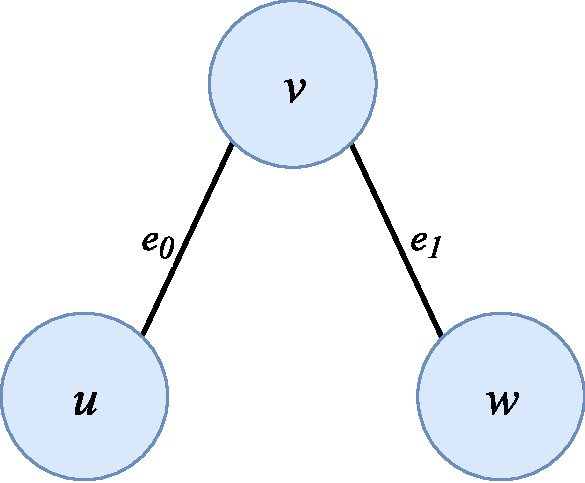
\includegraphics[scale=0.5]{grafo-simples}
\centering
\caption{Representação gráfica de G$_{1}$.}
\end{figure}

%%%%%
\subsection{Grafo Completo}
\label{conceitos__grafo--comleto}

Um \emph{grafo completo} G é um grafo onde cada par de vértices é conectado por uma aresta, ou seja, $|E[G]| = \frac{n(n-1)}{2}$, que é o número máximo de arestas que um grafo pode ter, onde \emph{n} = |V[G]|.

\begin{figure}[H]
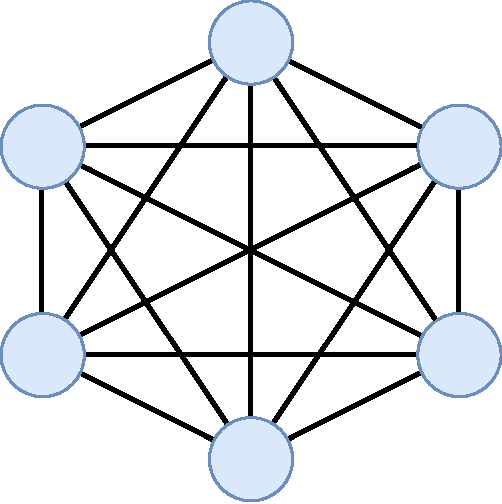
\includegraphics[scale=0.4]{grafo-completo}
\centering
\caption{Representação gráfica de um grafo completo.}
\end{figure}

%%%%%
\subsection{Clique}
\label{conceitos__grafo--clique}

Uma \emph{clique} C em um grafo G é um subconjunto de vértices tais que cada par de vértices do subconjunto é conectado por uma aresta. Isso significa dizer C que é um \emph{subgrafo} de G, $C \subseteq G$, e que C é completo, ou seja, $|E[C]| = \frac{n_{c}(n_{c}-1)}{2}$, onde $n_{c}$ = |V[C]|.

\begin{figure}[H]
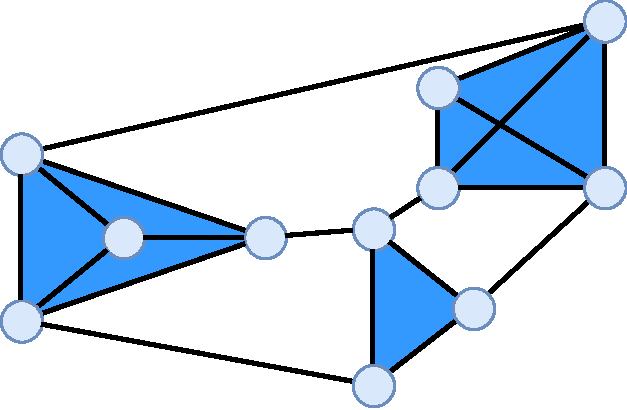
\includegraphics[scale=0.4]{grafo-clique}
\centering
\caption{Representação gráfica de um grafo com cliques, onde cada área colorida representa uma clique}
\end{figure}

%%%%%
\subsection{Grau de um vértice}
\label{conceitos__grafo--grau}

\def \variable {\emph{v}}

O \emph{grau} de um vértice \emph{v} em um grafo G, denotado por \emph{d$_{G}$}(\emph{v}), é o número de arestas em G que incidem sobre \emph{v}. De modo particular, \emph{d$_{G}$}(\emph{v}) é o número de vizinhos de \emph{v} em G. Um vértice de grau zero é chamado de \emph{vértice isolado}. O grau mínimo e o grau máximo dos vértices de G são denotados por $\delta(G)$ e $\Delta(G)$, respectivamente, enquanto que \emph{d}(G) denota seu \emph{grau médio}, $\frac{1}{n}\sum_{v\in V}(d(v))$, onde \emph{n} é o número de vértices de G~\cite{bondy1976graph}.

%%%%%
\subsection{Peso}
\label{conceitos__grafo--peso}

Grafos são muito utilizados para modelar problemas reais e, em certos problemas, é preciso incluir alguns atributos especiais, como por exemplo um custo, que está associado com as arestas. Em uma rede de tráfego, por exemplo, esse custo poderia representar a distância entre dois lugares. Esses problemas costumam ser modelados por um grafo ponderado.

Para cada aresta \emph{e} de um grafo G, é associado um número real \emph{w}(\emph{e}), denominado \emph{peso}. Sendo assim, G, com o atributo peso associado as arestas, é chamado de \emph{grafo ponderado}.

%%%%%

\subsection{Componente}
\label{conceitos__grafo--componente}

Um grafo é dito \emph{conexo} se, para cada par de vértices, existe um \emph{caminho} entre eles, ou seja, uma sequência de vértices onde cada par consecutivo na sequência é ligado por uma aresta.

Quando um grafo não é conexo, ele se divide em \emph{componentes}, que são subconjuntos de vértices desse grafo, onde cada par destes vértices possui um caminho entre eles, ou seja, a componente é conexa. Além disso, as componentes são isoladas, ou seja, não existe aresta ligando vértices de diferentes componentes.

\begin{figure}[H]
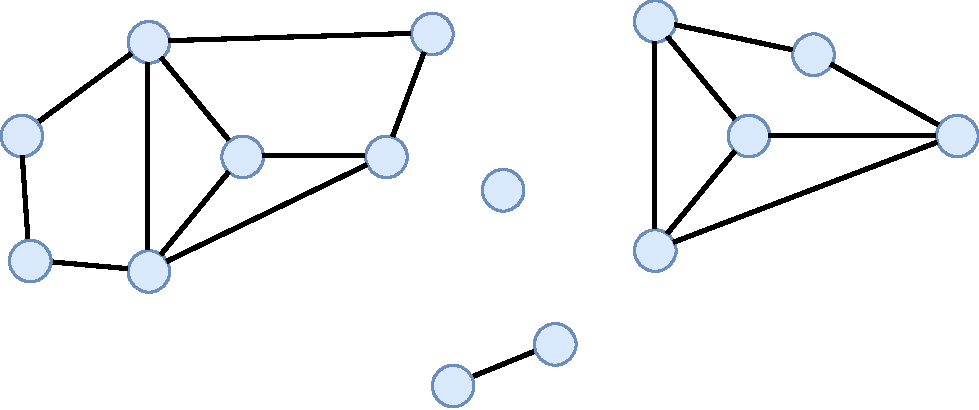
\includegraphics[scale=0.5]{grafo-componentes}
\centering
\caption{Grafo dividido em componentes. Note que um vértice isolado também pode ser visto como uma componente.}
\end{figure}

%%%%%
\subsection{Componente Gigante}
\label{conceitos__grafo--componente-gigante}

\emph{Componente gigante} é um termo informal utilizado para
um componente conexo que contém uma fração significativa de todos os vértices de um grafo. Além disso, quando um grafo contém um componente gigante, quase sempre este componente é único.

Na figura \ref{fig:grafo-componente-gigante}, é apresentado uma rede de relacionamentos românticos em uma escola secundária americana. É possível identificar uma componente gigante, onde até estudantes com apenas uma relação estão incluídos nela. Também é fácil perceber que, basta que uma pessoa de uma das componentes menores ter um relacionamento com alguém da componente gigante, que todos os vértices desta componente passarão a fazer parte da componente gigante.

É por este motivo que, quase sempre, uma componente gigante é única em uma rede, pois basta uma aresta de uma componente a outra para que elas se unam, formando uma nova componente única.

\begin{figure}[H]
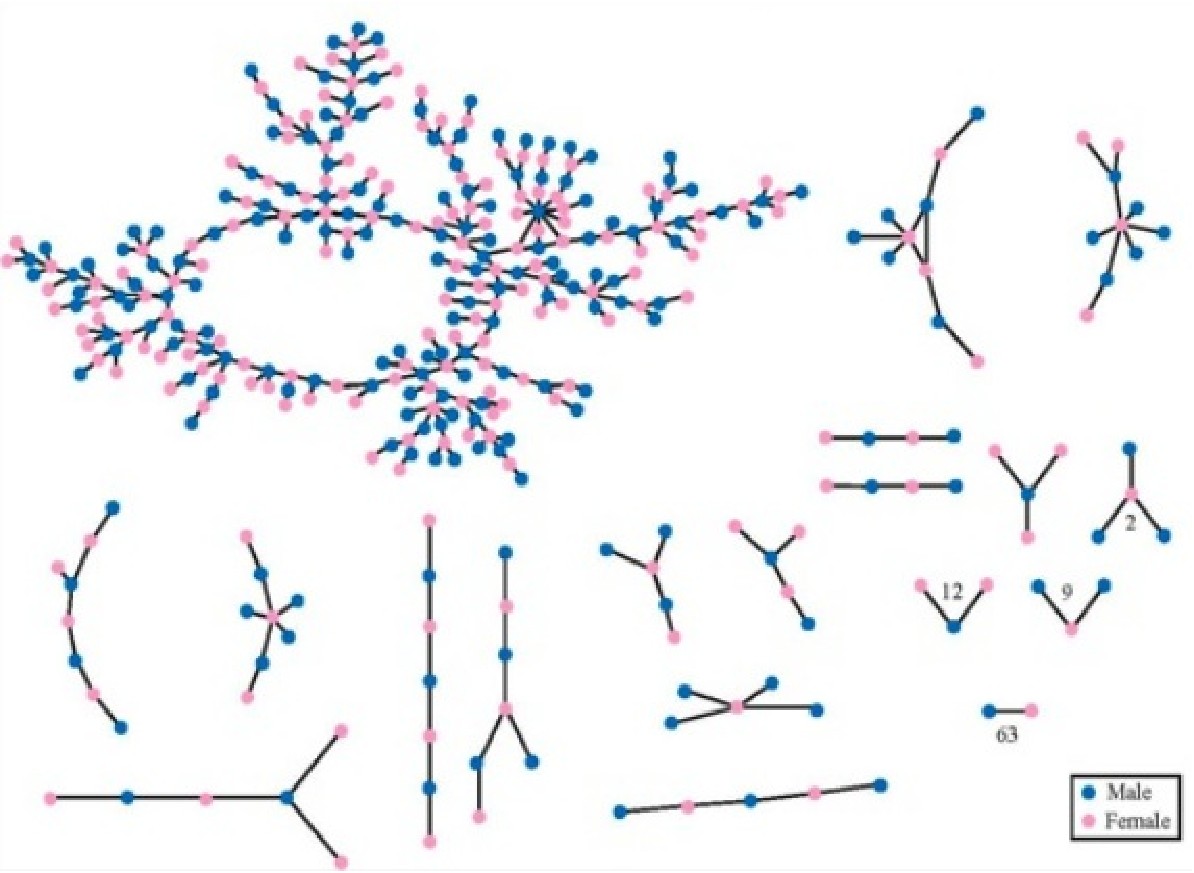
\includegraphics[scale=0.6]{grafo-componente-gigante}
\centering
\caption{
    Rede de relacionamentos românticos em uma escola secundária americana num período de 18 meses. Fonte:~\cite{bearman2004chains}
}
\label{fig:grafo-componente-gigante}
\end{figure}

%%%%%%%%%%%%%%%%%%%%%%%%%%%%%%%%%%%%%%%%%%%%%%%%%%%%%%%%%%%
\section{\texorpdfstring{\MakeUppercase{Fechamento Triádico}}{}}
\label{conceitos__fechamento-triadico}

Na maioria dos estudos de redes sociais, é interessante entender como uma rede evolui através do tempo. O \emph{fechamento triádico} é um princípio básico que auxilia esse entendimento, através da formação de novas arestas.

Claro que as alterações que as arestas de uma rede podem sofrer dependem muito do tipo de rede que está sendo analisada, porém, o princípio do fechamento tríadico é definido basicamente da seguinte maneira:

\begin{quotation}
    \emph{Se duas pessoas em uma rede social têm um amigo em comum, então há uma probabilidade maior de se tornarem amigos em algum momento do futuro}~\cite{rapoport1953spread}.
\end{quotation}

A figura \ref{fig:grafo-fechamento-triadico} ilustra exemplos de fechamentos triádicos. Os vértices \emph{A} e \emph{E} tem o vértice \emph{B} em comum, então a formação de uma nova aresta \emph{A}-\emph{E} produz uma situação onde os três vértices estão conectados. Essa estrutura de três vértices é chamada de \emph{triângulo}. O termo \emph{fechamento triádico} vem do fato de que a aresta \emph{A}-\emph{E} teve o efeito de ‘‘fechar’’ o terceiro lado deste triângulo. Neste exemplo, o mesmo comportamento ocorre com as arestas \emph{B}-\emph{F} e \emph{D}-\emph{G}.

Ao observar grandes redes sociais por um período de tempo, é comum identificar esse tipo de comportamento de fechamento triádico.

\begin{figure}
    \center
    \subfigure[fig:fechamento-triadico-antes][Antes de formar novas arestas]{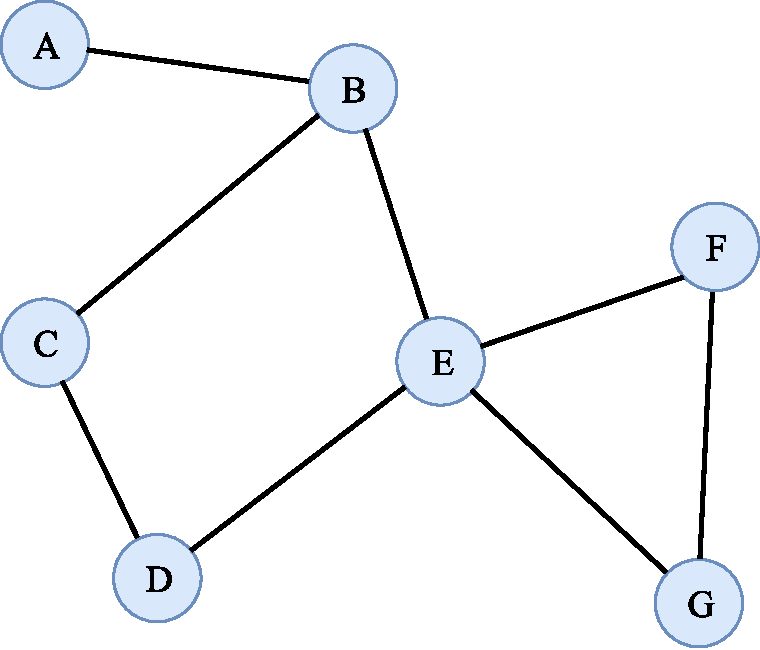
\includegraphics[width=6cm]{fechamento-triadico-antes}}
    \qquad
    \subfigure[fig:fechamento-triadico-depois][depois de formar novas arestas]{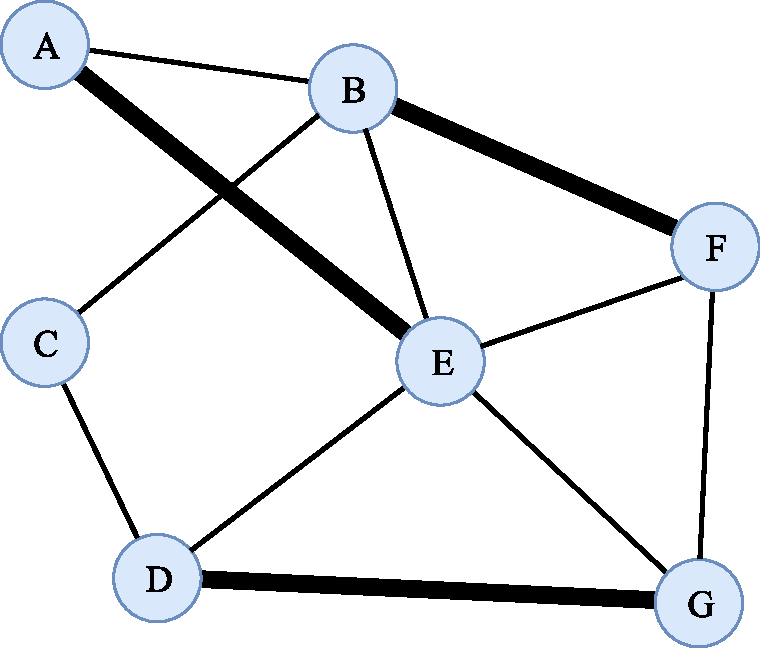
\includegraphics[width=6cm]{fechamento-triadico-depois}}

    \caption{Ao observar uma rede por um período de tempo, é possível ver que novas arestas são formadas, muitas vezes seguindo o princípio do fechamento triádico.}
    \label{fig:grafo-fechamento-triadico}
\end{figure}

%%%%%
\subsection{Coeficiente de clustering}
\label{conceitos__fechamento-triadico--coeficiente-clustering}

A regra do fechamento triádico motiva a definição de algumas métricas. Uma delas é o coeficiente de \emph{clustering}.

O \emph{coeficiente de clustering} de um vértice \emph{v} é a probabilidade de que dois de seus vizinhos, selecionados aleatoriamente, sejam conectados por uma aresta.

Na figura \ref{fig:grafo-fechamento-triadico}, por exemplo, o vértice \emph{E} possui coeficiente de \emph{clustering} $\frac{1}{6}$ antes da formação de novas arestas, pois, como \emph{E} tem 4 vizinhos, o número máximo de arestas que poderiam ser formadas entre eles é $\frac{4(4 - 1)}{2} = 6$, mas só existe uma. Após a formação de novas arestas, \emph{E} passa a ter um coeficiente de \emph{clustering} de $\frac{4}{10}$.

O \emph{coeficiente de clustering médio} é dado por $\frac{1}{n}\sum_{v\in V}(C_{v})$, onde $C_{v}$ é o coeficiente de \emph{clustering} do vértice \emph{v}.

\todo{Será que precisa colocar algo sobre coeficiente de clustering em grafo ponderado?}

\todo{ver depois:}

\url{https://arxiv.org/pdf/cond-mat/0311416.pdf}

\url{https://toreopsahl.com/tnet/weighted-networks/clustering/}

\url{http://citeseerx.ist.psu.edu/viewdoc/download?doi=10.1.1.139.9018&rep=rep1&type=pdf}

%%%%%%%%%%%%%%%%%%%%%%%%%%%%%%%%%%%%%%%%%%%%%%%%%%%%%%%%%%%
\section{\texorpdfstring{\MakeUppercase{Modularidade/comunidades}}{}}
\label{conceitos__modularidade}

Muitos dos problemas representados por uma estrutura de grafos apresentam \emph{comunidades} (ou \emph{clusters}), que podem ser definidas como subconjuntos de vértices que podem ser facilmente agrupados, pois são densamente conectados internamente, porém esparsamente conectados com o restante do grafo. Assim, é interessante identificar estas comunidades para analisá-las separadamente, pois podem ter diferentes propriedades, tais como grau dos vértices, coeficiente de \emph{clustering}, centralidade, etc.

\emph{Modularidade} é a medida que busca a divisão de um grafo em comunidades. Quanto maior a modularidade de um grafo, maior a densidade nas conexões entre vértice de uma mesma comunidade.

%%%%%%%%%%%%%%%%%%%%%%%%%%%%%%%%%%%%%%%%%%%%%%%%%%%%%%%%%%%
\section{\texorpdfstring{\MakeUppercase{Partidos Políticos no Brasil}}{}}
\label{conceitos__partidos-brasil}

Definição de Partidos Políticos no Brasil

Podemos entender, assim, que o partido político, como pessoa jurídica de direito privado, é um grupo social de relevante amplitude, destinado à arregimentação coletiva, em torno de ideias e de interesses, para levar seus membros a compartilhar do poder decisório nas instâncias governamentais~\cite{michels2010direito}.

(MICHELS, Vera Maria Nunes. Direito Eleitoral. 3. ed. Porto Alegre: Livraria do Advogado, 2004, p. 151)


%%%%%%%%%%%%%%%%%%%%%%%%%%%%%%%%%%%%%%%%%%%%%%%%%%%%%%%%%%%

\section{\texorpdfstring{\MakeUppercase{Coligações}}{}}
\label{conceitos__coligacoes}

Definição de Coligações

\todo{além de definir uma coligação, dizer que no trabalho falamos sobre "um partido fazer coligação com outro" como forma de dizer que "os dois partidos pertencem a uma mesma coligação"}

%%%%%%%%%%%%%%%%%%%%%%%%%%%%%%%%%%%%%%%%%%%%%%%%%%%%%%%%%%%

\section{\texorpdfstring{\MakeUppercase{Espectro Político}}{}}
\label{conceitos__espectro-politico}

Definição de Espectro Político: Esquerda x Direita

A esquerda é o espectro ideológico que pretende empoderar grupos sub-representados nas esferas de
poder; e
A direita é o espectro ideológico que pretende preservar ou ampliar os poderes de grupos já devidamente
representados nas esferas de poder.

SILVA, G. J. . Conceituações Teóricas: Esquerda e Direita. Humanidades em Diálogo (Impresso) , v. VI, p. 149-162, 2014


%%%%%%%%%%%%%%%%%%%%%%%%%%%%%%%%%%%%%%%%%%%%%%%%%%%%%%%%%%%

\section{\texorpdfstring{\MakeUppercase{Visualizações}}{}}
\label{conceitos__visualizacoes}
\subsection{Gephi}
\label{conceitos__visualizacoes--gephi}

\todo{Explicar sobre o Gephi}

\subsection{Layouts}
\label{conceitos__visualizacoes--layouts}

\todo{Fazer uma subsection para cada layout do gephi que utilizarmos}
